Interaction between human and complex cyber-physical systems is an essential aspect of modern computing platforms. These interactions enable users to provide inputs to software systems and services and interpret computation output. Over the last half a century~\cite{hci_history_1,hci_history_2}, researchers in academia and industry spent a significant effort to make this interaction as effortless as possible. Input-output (IO) peripherals and complex user interfaces (UI) are keys to facilitate this interaction. Intuitive UIs were quintessential to the widespread deployment of computing devices around us and the rapid adoption of remote applications and services. 

Security and safety-critical remote applications such as e-voting, online banking, industrial control systems (such as remote PLCs~\cite{controlbyweb}), and medical devices~\cite{medicalDevice} rely upon user interaction. This is typically performed through a \emph{host} system that generally is a standard $x86$ platform, which gives the host access to the raw IO data that is exchanged between the user and the remote server. The host consists of large and complex software systems such as the operating system, hypervisor, device drivers, applications such as a browser, and a diverse set of hardware components that expose the host to a large attack surface. Due to cost and convenience, general-purpose PCs are prevalent in many safety-critical application domains such as industrial plants and hospitals. For example, the WannaCry ransomware incident showed that NHS hospitals relied on Windows XP platforms~\cite{berry_2017,field_wannacry_2018} despite the fact that Microsoft ended the mainstream support in 2009~\cite{xp_support}. During the current Covid-19 pandemic, we have seen a steady rise of working from home~\cite{covid_work}. In such a scenario, most of the users access these remote systems through their standard desktops and laptops.


\begin{figure}[t]
  \centering
    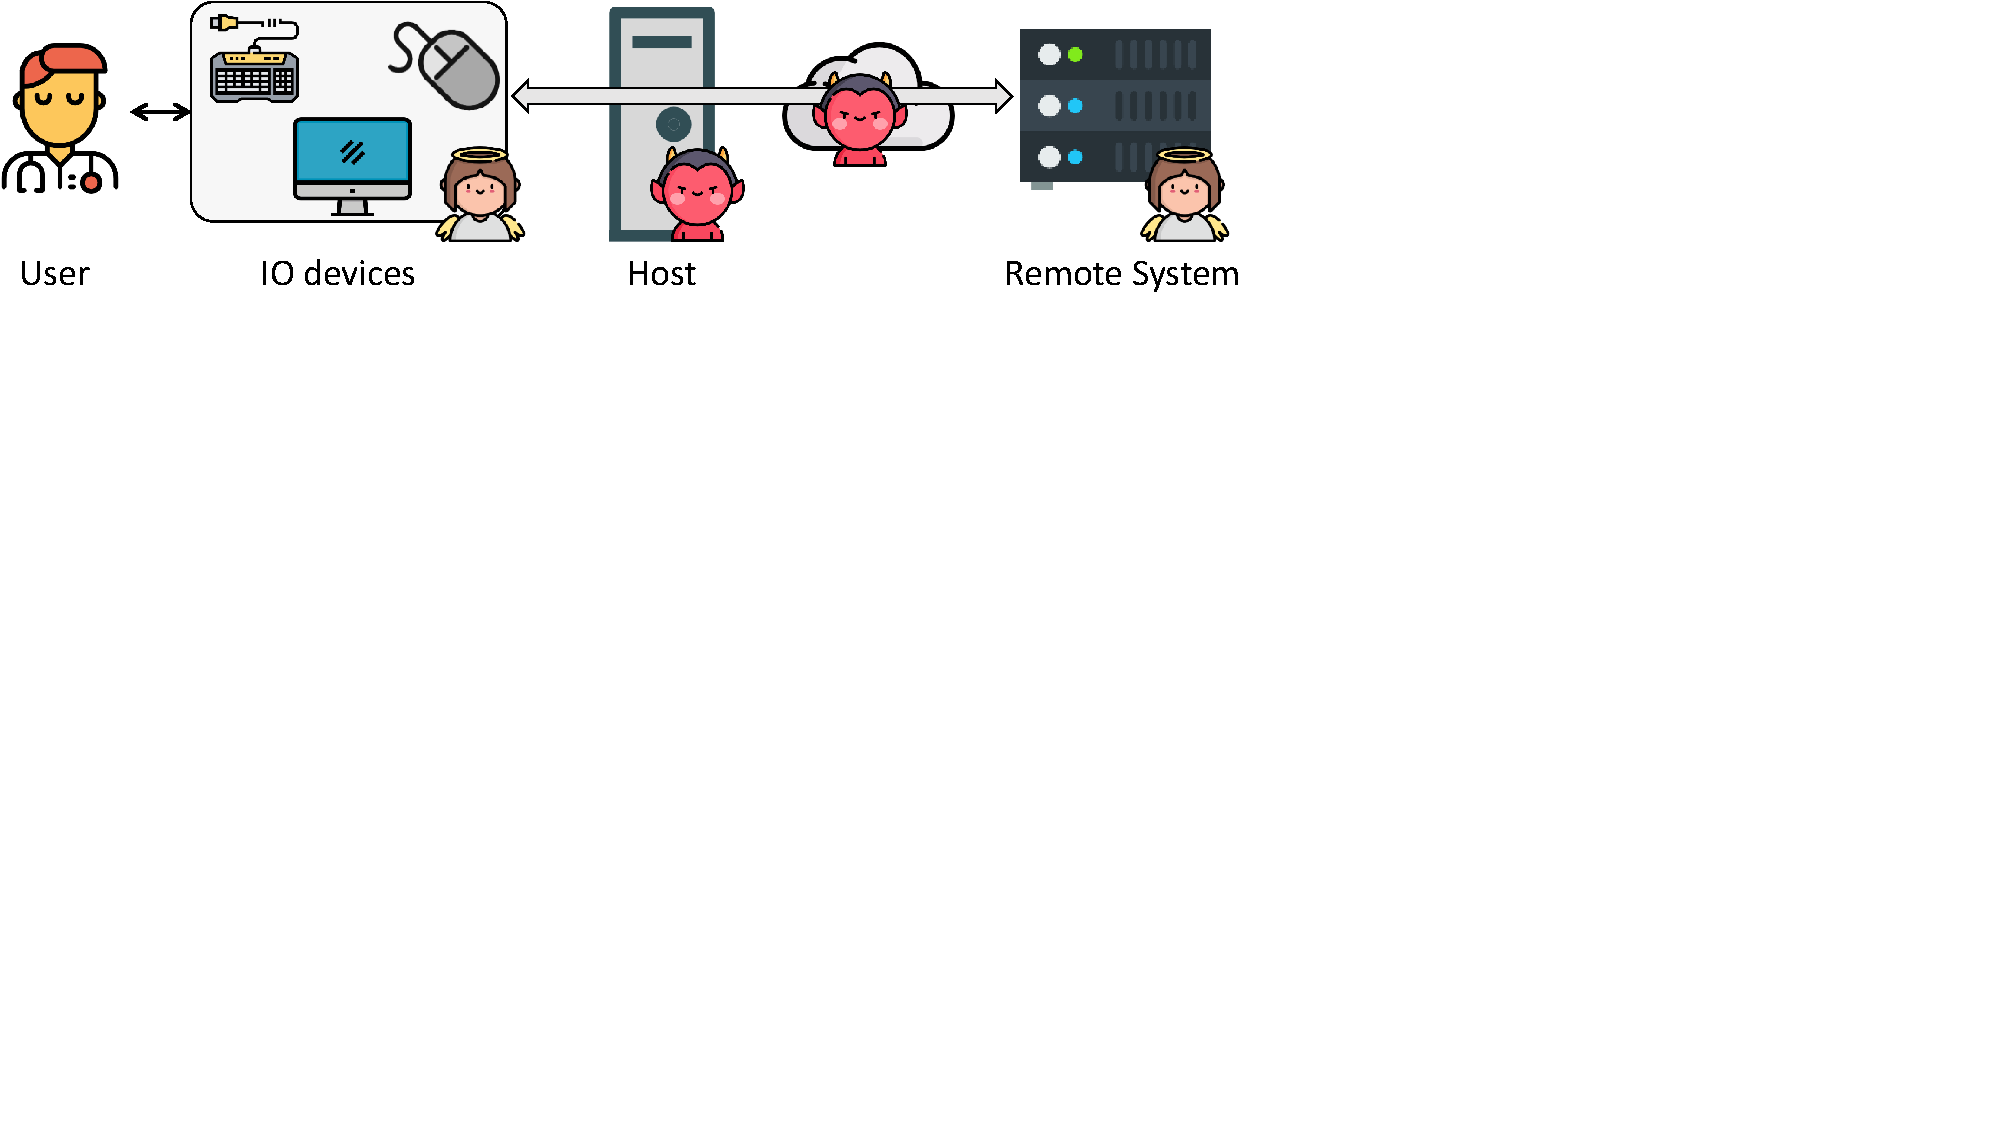
\includegraphics[trim={0 14cm 12cm 0},clip,width=\linewidth]{chapters/introduction/images/trustedPath.pdf}
    \caption[Remote trusted path through untrusted host]{\textbf{Remote trusted path through untrusted host.} The user interacts with a remoter service (that is trusted) with her trusted IO peripherals through the untrusted host and network. A remote trusted path must ensure the integrity (and in some application scenarios, confidentiality) of the data between the user and the remote server.}
    \label{fig:trustedPath}
\end{figure}

\section{Trusted Path}
\label{ch:intro:trustedPath}

\emph{Trusted path} provides a secure channel between the user (specifically through the human interface devices - HIDs) and the end-point, typically a trustworthy application running on the host. A trusted path ensures that user inputs reach the intended application unmodified, and all the outputs presented to the user are generated by the legitimate application. Hence, a trusted path ensures \emph{IO integrity}. In certain scenarios, the trusted path also provides \emph{confidentiality} to the user data. Trusted path can also be extended to general peripherals such as accelerators, GPUs, and sensors, and even remote systems. Trusted path could be extended to a remote system where the user communicates with a remote end-point using the local host as an untrusted transport. An attacker who exploits the software stack, i.e., the hypervisor or the OS and/or the hardware (refer to~\Cref{fig:trustedPath}), can control the user's computer. Such an attacker can \emph{observe} and \emph{modify} any user interaction data without being detected by the user or the server, hence undermining the trusted path's properties. 

Trusted path to the local host is a well-researched area where many solutions focus on using trusted software components such as a trusted hypervisor~\cite{zhou2012building} or external trusted hardware~\cite{filyanov2011uni,weigold2011secure,McCPerRei2006,mannan2007using,Fidelius}. However, hypervisors are hard to deploy, have a large TCB, and are impractical in real-world scenarios as most of the existing verified hypervisors offer a minimal set of features, and some of the external device-based approaches such as transaction confirmation devices~\cite{filyanov2011uni,weigold2011secure} suffer from poor usability, security issues due to user habituation~\cite{anderson2016warning} and are only limited to simple inputs.


\section{Trusted Execution Environments (TEE)}

\emph{Trusted execution environments (TEEs)} such as Intel SGX, AMD SEV, ARM TrustZone, RISC-V keystone, etc., drastically reduce the trusted computing base (TCB) and provide security to applications, known as enclaves, without having to trust the operating system and hypervisor~\cite{costan2016intel,winter2008trusted,costan2016sanctum}. Thus, the attack surface is reduced by eliminating two of the largest sources of vulnerabilities for a system~\cite{checkoway2013iago,suzaki2011memory}. TEEs use \emph{isolation} primitives provided by the CPU to exclude all software but a single target application (commonly known as an enclave) from the software trusted computing base (TCB). Only the CPU is part of the hardware TCB, while the remaining hardware in the system is considered untrusted. Even memory is not included in the TCB and can only be used in conjunction with memory encryption and integrity protection. Such a trust model makes the TEEs ideal candidates for the aforementioned trusted path applications where the software stack is attacker-controlled. 

Apart from isolation from the OS, another crucial security primitive of TEEs is \emph{remote attestation}. A remote verifier can ensure that a (legitimate) platform is running an enclave with the correct code. In a simplified form, at the end of a remote attestation process, the platform generally\footnote{There exist some differences between remote attestation mechanisms in different TEE technologies. We use Intel SGX as an example here, and more details are provided in~\Cref{ch:background:SGX:attestation}. However, other approaches to remote attestation are comparable.} produces three following pieces of information to the verifier: 
\begin {enumerate}
\item A \emph{measurement} (cryptographic hash of the code and data) of the enclave to ensure that it is running the proper enclave code. The measurement is signed (\emph{report}) by the platform's attestation key that is physically bound to the platform. 
\item A successful verification of the signed measurement~\footnote{The verification is carried out by Intel Attestation Server.} ensures that the attestation key originates from a \emph{legitimate platform}.
\item The \emph{public key} of the platform that the remote verifier can use to establish a secure channel to provision secrets to the enclave.
\end{enumerate}

\myparagraph{Relay Attack on remote attestation} While SGX's remote attestation guarantees that the attested enclave runs the expected code, it \emph{does not}, however, guarantee that the enclave runs on the expected computing platform. An attacker that controls the software stack (OS, hypervisor, etc.) on the target platform can relay incoming attestation requests to another platform. This way, the user ends up attesting to the attacker's platform rather than her own. Relay attack enables the attacker to see all the IO data to and from the user, e.g., sensitive user input on display, and execute a long-term physical side-channel attack. Hence, relay attacks on Intel SGX remote attestation pose a real threat to trusted paths. Relay attack is not only limited to Intel SGX but also other comparable TEEs such as AMD SEV or RISC-V keystone. Note that the relay attack is a long-standing open problem in trusted computing, as already a decade ago, Parno identified it in the context of TPM attestation~\cite{parno2008bootstrapping}. Hence, directly incorporating a trusted path to a TEE like Intel SGX is not a trivial issue.


\myparagraph{Issues with trusted path} Solving the relay attack still does not make TEEs ideal for a trusted path. TEEs cannot communicate with any external device without going through the untrusted operating system. This results in a static hardware TCB from the enclave's perspective as the enclaves need to trust the OS/hypervisor, all the device drivers running on it, and all the external devices, even in a scenario where the enclave needs to communicate with only one external device. Lack of isolation, a vulnerability in one device driver, may allow the attacker to gain control over other devices\footnote{This property is also known as \emph{fault isolation}.}. Hence, constructing trusted path using existing TEEs results in a massive increment in both software and hardware TCB, nullifying the core advantage of using TEEs.


\myparagraph{Static software/hardware TCB} Static software/hardware TCB in TEEs is also critical in the modern data center where trusted path expands beyond simple IO operation. For example, users can deploy an application that uses sensitive medical data for training machine learning models on a GPU. Existing TEEs protect applications (enclaves) running on the CPU cores; however, they do not protect applications running on the external hardware, which in this case is a GPU. More and more applications rely on application-specific hardware devices (also known as accelerators) that are tuned for specific workloads. Such accelerators provide massive speedups over CPUs. The cloud providers move to a new breed of computing model to cope with such workloads and optimize flexible resource allocation\footnote{Resources such as CPU cores, memory, storage, network interface, etc., are allocated to the VM from a pool based on the demand. One such example is Amazon EC2~\cite{ec2} where storage and network interface is allocated to a VM dynamically.}. Such a model is known as the \emph{disaggregated} computing model~\cite{disaggregatedcomp}. Unlike the traditional CPU-centric computational model, where the CPU is the platform's sole executioner, in modern data centers, CPUs become mere coordinators of these special-purpose devices. The isolation and attestation primitive of traditional TEEs are geared towards the CPU-centric models as enclaves are running solely on the CPU cores, and only the CPU package is trusted. Hence the current TEE primitives such as the isolation and the attestation need redesigning to support the trusted path applications in the modern disaggregated cloud data centers.